\section{Introduction}

\subsection{Background and Motivation}

Urban emergency response is a core urban-informatics problem because access to public services is both spatially unequal and time-sensitive; the choice of accessibility measure can materially change conclusions about equity~\cite{talen1998,pereira2017equity}. Open data can improve accountability, but denominators, missing values, spatial disclosure control, and operational caveats can still make a simple map look more authoritative than its evidence allows. LFB publishes detailed incident records~\cite{lfb_incidents} and a six-minute first-pump attendance standard~\cite{lfb_attendance}. Earlier public-facing LFB visualisations include a GOV.UK performance prototype and the ODI station-closure map~\cite{govuk2014,odi2013}; both predate the present 2024--2026 window and neither exposes response-time denominators and coordinate completeness together. The 293{,}646-incident slice used here therefore motivates a current, auditable visual-analytics view in which response patterns and their limitations remain visible together.

Initial exploratory analysis of the most recent 26 months of LFB incident data (January 2024--February 2026, 293{,}646 records) confirms three motivating problems for this project:

\begin{itemize}
    \item \textbf{A consistent service-equity gap.} 32.4\% of incidents with recorded first-pump attendance time exceed the published six-minute benchmark~\cite{lfb_attendance}. The highest recorded-time exceedance shares are in outer-London boroughs including Hillingdon (52.2\%), Bromley (47.6\%), and Richmond upon Thames (45.2\%), while several inner-London boroughs sit below the London-wide reference line.
    \item \textbf{A resource-utilisation question.} False alarms account for 46.5\% of incidents and consume more pumps per incident on average (1.9) than fires (1.7). This workload can alter how borough response rankings are interpreted, so it must be available as a filter and sensitivity check rather than hidden inside the total.
    \item \textbf{A spatial data-quality problem.} Only 37.9\% of records carry precise coordinates; the remainder are available through a rounded coordinate family in the LFB release~\cite{lfb_incidents}. Street-level analysis must therefore expose coordinate completeness rather than silently treating the precise subset as the full incident population (\S\ref{sec:background-granularity}).
\end{itemize}

These motivating numbers are summarised in Table~\ref{tab:motivation}; the data conventions behind them are stated in \S1.4.

\begin{table}[h]
\centering
\small
\begin{tabularx}{\textwidth}{lll}
\toprule
Metric & Value & Interpretation \\
\midrule
Total incidents (Jan 2024 -- Feb 2026) & 293{,}646 & Dataset scope \\
First-pump attendance $>$ 6 minutes & 32.4\% & Service-equity motivation \\
False alarms (share of all incidents) & 46.5\% & Resource-utilisation question \\
Records with precise (non-suppressed) coordinates & 37.9\% & Spatial-analysis limitation \\
\bottomrule
\end{tabularx}
\caption{Motivating descriptive statistics computed by the author from LFB Incident Records~\cite{lfb_incidents}; \S1.4 specifies the field definitions.}
\label{tab:motivation}
\end{table}

\begin{figure}[H]
\centering
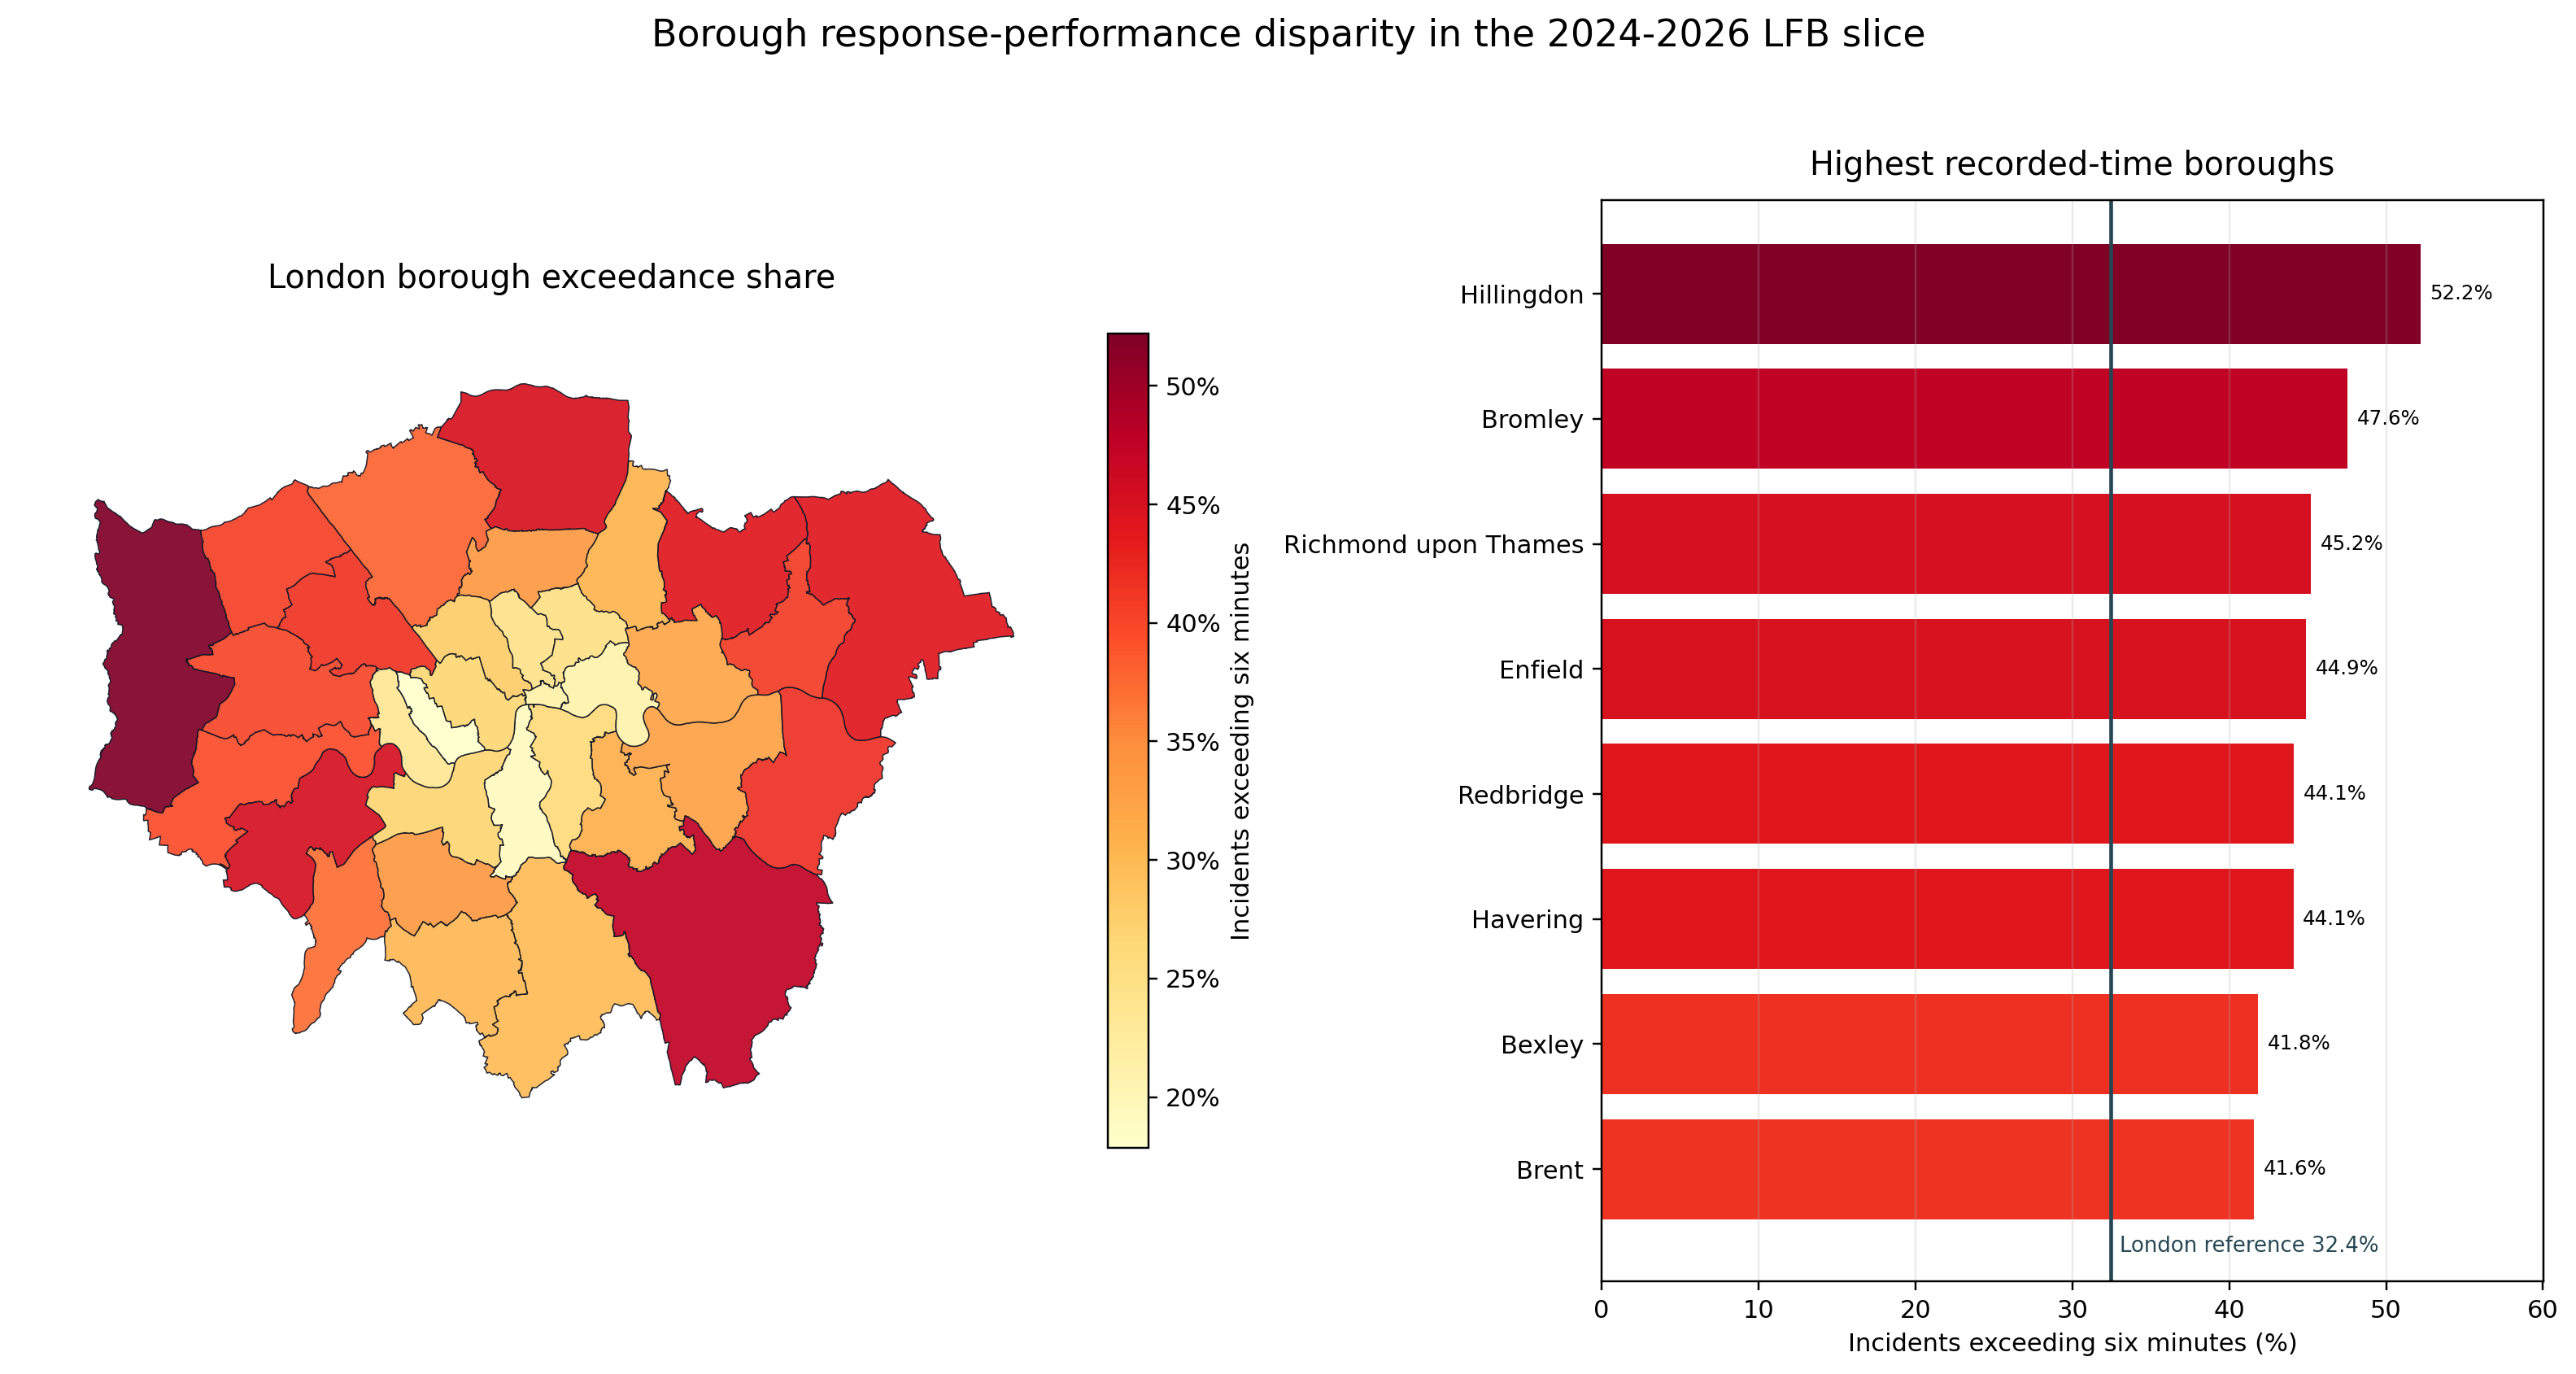
\includegraphics[width=\textwidth]{figures/early_context/fig_motivation_borough_exceedance_map.png}
\caption{Motivating borough-level response-performance gap, calculated by the author from LFB Incident Records~\cite{lfb_incidents}. The vertical line marks the project-wide recorded-time exceedance share.}
\label{fig:motivation-borough-exceedance-map}
\end{figure}

Together, these measured gaps and the limitations of earlier public-facing tools frame the project's contribution.

\subsection{Aims and Objectives}

The project aim is to design, build, and evaluate a web-based interactive visual analytics dashboard that helps users ask more defensible questions of LFB open data: where workload and response-time pressure appear together, how strongly those patterns depend on incident type and time, and what caveats are required before a map is interpreted as operational evidence. The dashboard targets two \emph{potential} stakeholder profiles: (a) LFB and Greater London Authority planners exploring borough-level evidence for discussion, and (b) academic and policy researchers studying urban emergency response equity. Operational adoption by either group is outside this project's scope; evaluation is limited to usability and analytical interpretability rather than operational decision validation (\S4.6).

The concrete objectives are:

\begin{enumerate}
    \item \textbf{Data pipeline.} Build a reproducible processing pipeline over LFB incident records, ONS borough boundaries, mobilisation records, and a public fire-station address list (postcode-geocoded for proximity context) that handles the 62\% missing-coordinate problem explicitly.
    \item \textbf{Spatial-temporal analytics.} Implement borough-level aggregations, diagnostic hexbin/density maps for the geocoded subset, and response-time distributions sliced by hour, weekday, borough, and incident type.
    \item \textbf{Interactive dashboard.} Deliver a Flask + D3.js dashboard with linked-view brushing across map, time-series, distribution, and ranking panels, plus a bounded station-proximity/assignment-footprint evidence strand that is explicitly framed as exploratory context rather than an operational dispatch, routing, coverage, or relocation model.
    \item \textbf{Evaluation.} Evaluate the artefact against the research questions below using a closed heuristic walk-through, scripted think-aloud/probe instruments, dashboard screenshots, and a compact think-aloud summary.
\end{enumerate}

\subsection{Research Questions}

The initial project brief listed five example questions. This thesis consolidates them into one primary research question and three supporting questions. The three-question form keeps the brief's spatial, temporal, visual-analytics, resource-context, and data-quality themes visible while avoiding a scattered evaluation chapter.

\begin{enumerate}
    \item \textbf{Primary RQ.} How can an uncertainty-aware visual analytics dashboard support structured inspection of London Fire Brigade incident demand and first-pump response performance using public open data?
    \item \textbf{RQ1.} Which boroughs, incident groups, and time periods show persistent incident demand or six-minute first-pump attendance exceedance patterns in the 2024--2026 LFB open-data slice?
    \item \textbf{RQ2.} How do mobilisation records, false-alarm workload, coordinate suppression, missing response times, and station-address evidence qualify the interpretation of those patterns?
    \item \textbf{RQ3.} To what extent do the linked dashboard and report evidence package help users make useful but qualified analytical judgements without overstating station coverage, routing, or relocation claims?
\end{enumerate}

The questions have distinct evidential roles. RQ1 is descriptive: borough-month and incident-group summaries establish where patterns persist. RQ2 is a qualification question: mobilisation matching, false-alarm sensitivity, response-time missingness, coordinate coverage, and station-address evidence test how far those descriptions can be trusted. RQ3 evaluates the artefact rather than London itself: linked-view behaviour, the heuristic walk-through, and task/probe evidence test whether users can reach a comparison while retaining the stated caveats. The primary RQ is answered only by synthesising these three strands; none supports routing, dispatch, forecasting, or relocation claims.

\subsection{Data Sources and Conventions}

The primary dataset is the \textbf{LFB Incident Records} open dataset \cite{lfb_incidents} published on the London Datastore, used here as the 2024-01 to 2026-02 slice (293{,}646 rows $\times$ 39 columns, 63\,MB). The implementation also uses the ONS / GLA borough boundary layer \cite{ons_boundaries}, LFB mobilisation records \cite{lfb_mobilisations}, incident-derived borough and station footprint centroids, and a London Datastore public fire-station address list \cite{lfb_stations} whose postcodes are geocoded for a bounded station-proximity check in \S5.6. The address list is not treated as a routing-grade station entrance dataset. All currently-used data are open and require no institutional access.

The descriptive statistics quoted in \S1.1 were computed directly from this slice. Response-time exceedance is the \texttt{FirstPumpArriving\_AttendanceTime} field exceeding 360 seconds~\cite{lfb_attendance}; precise coordinates are non-null \texttt{Easting\_m} / \texttt{Northing\_m} values within the Greater London bounding box; and borough medians exclude null and out-of-range entries. The reproducing notebook is \path{notebooks/01_initial_eda_executed.ipynb}. Because precise-coordinate suppression may vary by borough, incident type, or time, borough analysis uses the near-complete rounded family and the dashboard exposes per-borough precise-coordinate coverage (\S\ref{sec:background-granularity}).

\subsection{Methodology Overview}

The reported work followed a four-phase workflow:

\begin{itemize}
    \item \textbf{Phase 1} (April 2026, completed): data acquisition, exploratory analysis, literature review; closed at the Preliminary Report submission on 30 April 2026.
    \item \textbf{Phase 2} (May--June 2026, completed): dashboard implementation in Flask + D3.js with iterative internal review.
    \item \textbf{Phase 3} (July 2026, completed for this report): evaluation, usability testing, and performance profiling.
    \item \textbf{Phase 4} (post-report): presentation and any further code-release housekeeping outside the evidence assessed in this report.
\end{itemize}

Tooling: Python 3.12 (\texttt{pandas}, \texttt{GeoPandas}) for the analytic backend, D3.js v7~\cite{bostock2011} for client-side visualisation, Flask for the API layer, Git for version control, and Zotero for reference management.

\subsection{Report Structure}

The remainder of this report follows the assessment logic. \S\ref{sec:background} establishes the domain, data, and operating definitions; \S\ref{sec:literature} reviews prior work and derives the design gap; \S4 specifies the artefact; \S5 records its implementation; and \S6 evaluates the results against the research questions. \S7 covers legal, social, ethical, and professional issues, while \S8 concludes. Appendices A--C index reproducibility material and provide the dashboard user guide.
